% Template for PLoS
% Version 1.0 January 2009
%
% To compile to pdf, run:
% latex plos.template
% bibtex plos.template
% latex plos.template
% latex plos.template
% dvipdf plos.template

\documentclass[10pt]{article}

% amsmath package, useful for mathematical formulas
\usepackage{amsmath}
% amssymb package, useful for mathematical symbols
\usepackage{amssymb}

% graphicx package, useful for including eps and pdf graphics
% include graphics with the command \includegraphics
\usepackage{graphicx}

% cite package, to clean up citations in the main text. Do not remove.
\usepackage{cite}

\usepackage{color} 

% Use doublespacing - comment out for single spacing
%\usepackage{setspace} 
%\doublespacing


% Text layout
\topmargin 0.0cm
\oddsidemargin 0.5cm
\evensidemargin 0.5cm
\textwidth 16cm 
\textheight 21cm

% Bold the 'Figure #' in the caption and separate it with a period
% Captions will be left justified
\usepackage[labelfont=bf,labelsep=period,justification=raggedright]{caption}

% Use the PLoS provided bibtex style
\bibliographystyle{plos2009}

% Remove brackets from numbering in List of References
\makeatletter
\renewcommand{\@biblabel}[1]{\quad#1.}
\makeatother


% Leave date blank
\date{}

\pagestyle{myheadings}
%% ** EDIT HERE **

\usepackage[utf8]{inputenc}

%% ** EDIT HERE **
%% PLEASE INCLUDE ALL MACROS BELOW

%% END MACROS SECTION

\begin{document}

% Title must be 150 characters or less
\begin{flushleft}
{\Large
\textbf{Low-Level Fusion of Stereo Vision and ToF Range Sensors\\
		- A State of the Art Research}
}
% Insert Author names, affiliations and corresponding author email.
\\
Nick Schneider$^{1}$
\\
\bf{1} Nick Schneider RD/FFU, Daimler AG, Böblingen, BW, Germany
\\
$\ast$ E-mail: nick.schneider@daimler.com
\end{flushleft}

% Please keep the abstract between 250 and 300 words
%\section*{Abstract}

% Please keep the Author Summary between 150 and 200 words
% Use first person. PLoS ONE authors please skip this step. 
% Author Summary not valid for PLoS ONE submissions.   
%\section*{Author Summary}

\section*{Introduction}

Die Vorteile von Time-of-Flight Sensoren liegen in der Genauigkeit und der schnellen Bereitstellung der Entfernungsdaten. Nachteile haben diese Sensoren jedoch in der geringen Auflösung und dem eingeschränkten Objektverständnis. Stereokamerasysteme dagegen punkten mit einer hohen Auflösung und einer hohen Genauigkeit in der Winkelmessung. Zudem sind Kamerasysteme in der Lage über Lernalgorithmen und Featureextraktion Objekte hinsichtlich ihrer Klasse genauer zu spezifizieren. Nachteile von Stereosystemen liegen in der Berechnung der Entfernungsdaten, bei der die passive Triangulation über eine Korrespondenzsuche zwischen linkem und rechtem Bild erfolgt.

Eine Fusion von Time-Of-Flight-Sensoren und Stereokamera-Systemen liegt aus diesen Gründen nahe. Die Fusion kann dabei auf verschiedenen Ebenen erfolgen. In \cite{Haberjahn2010} wird zwischen Low-, Mid- und Highlevel Fusion unterschieden. Dabei versteht \cite{Haberjahn2010} unter Low-Level Fusion die Kombination der Rohdaten oder der kalibrierten und gefilterten Punkte der jeweiligen Sensoren. Low-Mid-Level Fusion betrachtet hingegen einen fusionierten Segmentierungsansatz, während Mid-Level die Fusion ganzer Segmente oder Objekte bearbeitet. Zuletzt werden bei der High-Level Fusion das Tracking oder die daraus resultierenden Trajektorien fusioniert. Eine Übersicht der Definition nach \cite{Haberjahn2010} findet sich in Figure \ref{img:haberjahn_sensorfusion}.

\begin{figure}[ht]\centering%[]%[H]
	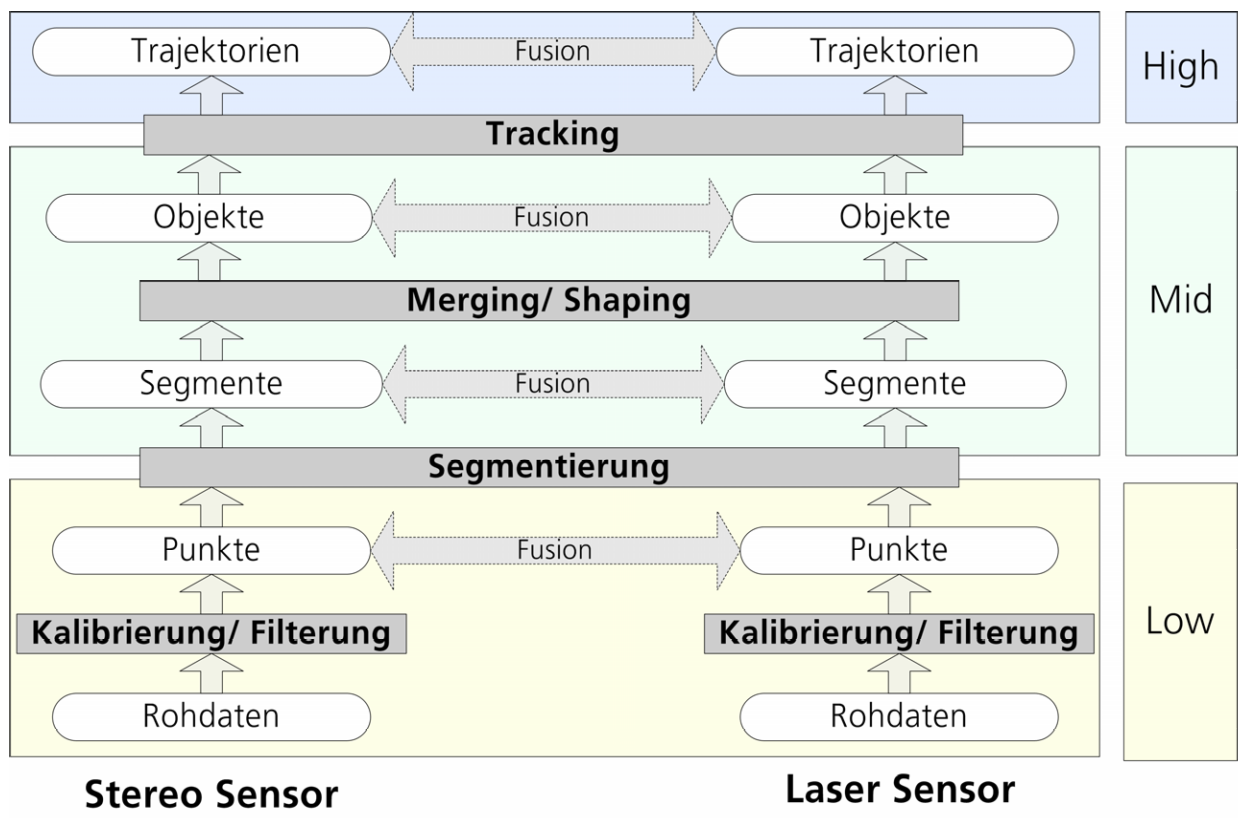
\includegraphics[width=15cm]{images/png/haberjahn_sensorfusion.png}
	\caption[Badino Interpolation]{ Vertikale und horizontale Interpolation. Die Farben kodieren die Entfernung \cite{Badino2011a} }.
	\label{img:haberjahn_sensorfusion}
\end{figure}

\section*{State of the Art}


\subsection*{Low-Level Sensor Fusion}

\subsubsection*{A Laserscanner-Vision Fusion System Implemented on the TerraMax Autonomous Vehicle, Broggi, A. \cite{Broggi2006}}

In \cite{Broggi2006} wird eine Low-Mid-Level Fusion eines 4-Ebenen-Laserscanners mit einem Stereokamerasystem vorgeschlagen. Dabei wird mit Hilfe der Stereokamera der Nickwinkel des Systems berechnet und damit die Laserscanner-Daten korrigiert. Des Weiteren wird eine Sensorfusion in einer "Bitmap" vorgeschlagen, welche im Endeffekt einer Art Occupancy Grid entspricht.
Bei der Berechnung des Nickwinkels stellt sich die Frage, inwiefern die dreidimensionale Rotationsmatrix berechnet wird. Im Paper macht es den Anschein, als würde lediglich der Nickwinkel berechnet werden, wodurch dennoch Probleme im Rollwinkel entstehen können.

\subsubsection*{Integrating LIDAR into Stereo for Fast and Improved Disparity Computation Badino, H. \cite{Badino2011a}}

\cite{Badino2011a} schlägt vor, die Vorteile von LIDAR und Stereo zu verbinden und dadurch deren Schwächen zu kompensieren. Während LIDAR zwar genau, die Repräsentation der Punkte jedoch spärlich ist, so punktet Stereo mit einer hohen horizontalen und vertikalen Auflösung, weist jedoch gerade in unstrukturierten Szenen oder Szenen mit wiederkehrenden Mustern deutliche Schwächen auf.
In \cite{Badino2011a} werden zwei Möglichkeiten für eine Low-Level Stereo/LIDAR Fusion vorgeschlagen:

\textbf{Disparity Space Reduction:} Zur Reduktion von Rechenzeit bei klassischen Stereoverfahren, werden sogenannte Disparitätsintervalle genutzt. Nach einer Rektifizierung werden Korrespondenzen des Pixels $(u,v)$ im rechten Bild zwischen den Pixeln $(u+d_{min},v)$ und $(u+d_{max},v)$ gesucht. 

Für die Berechnung von $d_{max}$ und $d_{min}$ werden in diesem Paper die im Vergleich zu Stereo präziseren LIDAR-Daten zunächst in ein dichtes Entfernungsbild transformiert. Dazu werden die LIDAR-Messungen in die Bildebene der linken Kamera projiziert und sowohl horizontal, als auch vertikal interpoliert (vgl. Figure \ref{img:badino_interpolation}).

\begin{figure}[ht]\centering%[]%[H]
	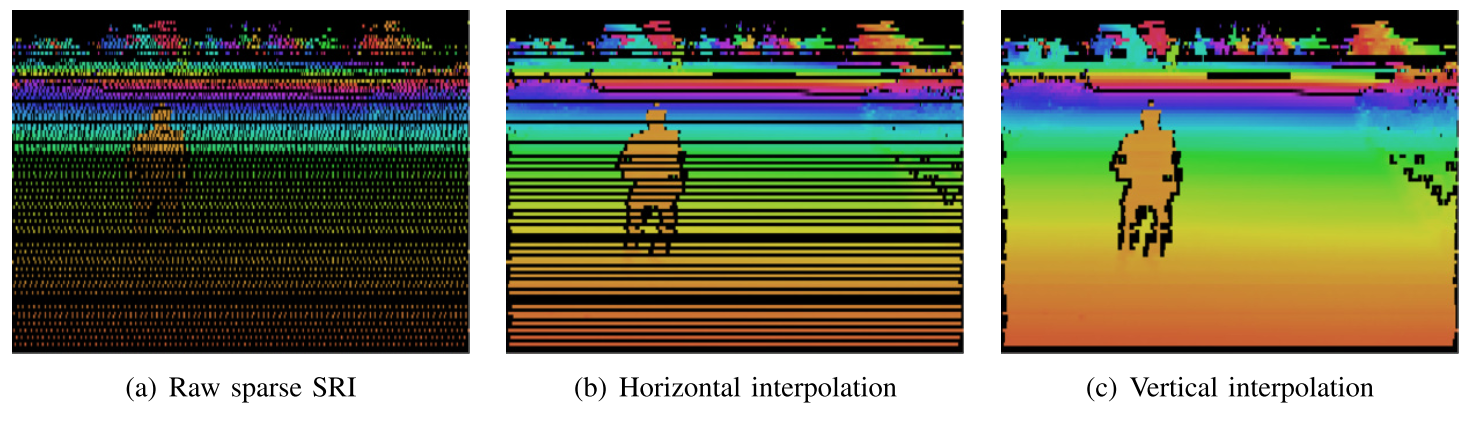
\includegraphics[width=15cm]{images/png/badino_interpolation.png}
	\caption[Badino Interpolation]{ Vertikale und horizontale Interpolation. Die Farben kodieren die Entfernung \cite{Badino2011a} }.
 	\label{img:badino_interpolation}
\end{figure}
Im Anschluss wird durch Erosion eine minimale und durch Dilatation eine maximale Distanz berechnet. Diese Distanzen werden wiederum in minimale/maximale Disparitäten $d_min$, $d_max$ transformiert und daraus über Korrespondenzsuche ein Disparitätsbild berechnet. Die Schritte sind in Figure \ref{img:badino_computation} verdeutlicht.

\begin{figure}[ht]\centering%[]%[H]
	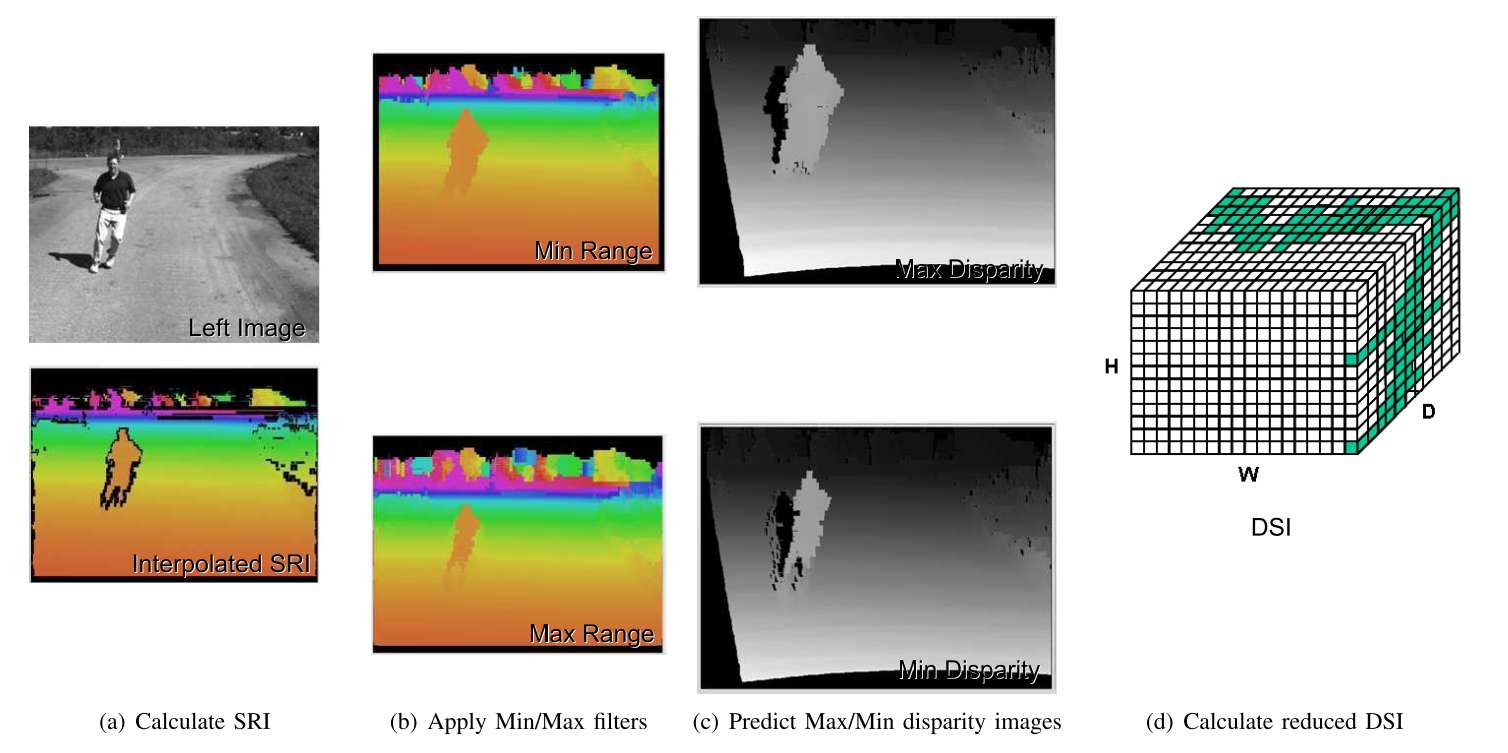
\includegraphics[width=15cm]{images/png/badino_dsi_computation.png}
	\caption[Reduziertes Disparitätsbild]{ Schritte zur Berechnung eines reduzierten Disparitätsbilds. \cite{Badino2011a} }.
	\label{img:badino_computation}
\end{figure}

\textbf{Path Promotion:} Neben der Reduktion des Suchraums schlägt \cite{Badino2011a} eine weitere Disparitätsberechnung durch Dynamic Programming vor. In die Kostenfunktion fließen die über den LIDAR berechneten, prädizierten Disparitäten, sowie der Gradient des prädizierten Disparitätsbilds mit ein.
Mögliche Verbesserungen dieses Algorithmus wäre die Erweiterung der einzeiligen Optimierung auf eine reduzierte globale Version von Dynamic Programming durch Semi Global Matching, welche in \cite{Hirschmuller2005} vorgestellt wird.

\subsubsection*{Fusion of time-of-flight depth and stereo for high accuracy depth maps Zhu, J. \cite{Zhu2008}}

\subsection*{Mid-Level Sensor Fusion}

Hier folgt der Teil zur Mid-Level Fusion
% You may title this section "Methods" or "Models". 
% "Models" is not a valid title for PLoS ONE authors. However, PLoS ONE
% authors may use "Analysis" 
%\section*{Materials and Methods}

% Do NOT remove this, even if you are not including acknowledgments
%\section*{Acknowledgments}


%\section*{References}
% The bibtex filename
\bibliography{mendeleybib}

%\section*{Figure Legends}
%\begin{figure}[!ht]
%\begin{center}
%%\includegraphics[width=4in]{figure_name.2.eps}
%\end{center}
%\caption{
%{\bf Bold the first sentence.}  Rest of figure 2  caption.  Caption 
%should be left justified, as specified by the options to the caption 
%package.
%}
%\label{Figure_label}
%\end{figure}


%\section*{Tables}
%\begin{table}[!ht]
%\caption{
%\bf{Table title}}
%\begin{tabular}{|c|c|c|}
%table information
%\end{tabular}
%\begin{flushleft}Table caption
%\end{flushleft}
%\label{tab:label}
% \end{table}

\end{document}

